\providecommand{\home}{../../..}
\documentclass[\home/main.tex]{subfiles}
\usetikzlibrary[arrows,snakes,backgrounds]
\usetikzlibrary{calc,positioning,fit}

\begin{document}

% \begin{sidewaysfigure}
\begin{tikzpicture}
    \def\picMinWidth{3cm}
    \def\picMinHeight{3.0cm}

    \tikzset{
        block/.append style={node distance=7.5mm,minimum width=3.5cm},
        subblock/.style={block, minimum width=1.5cm},
        picture/.style={block, node distance=6cm, fill=white, draw=white,minimum width=\picMinWidth, minimum height=\picMinHeight, text width=\picMinWidth,},
        preSpacedDash/.style={preSpaced, dashed,draw=black!50, thin},
        annot/.style={text width=4em, text centered},
    }

    \node[block] (env) {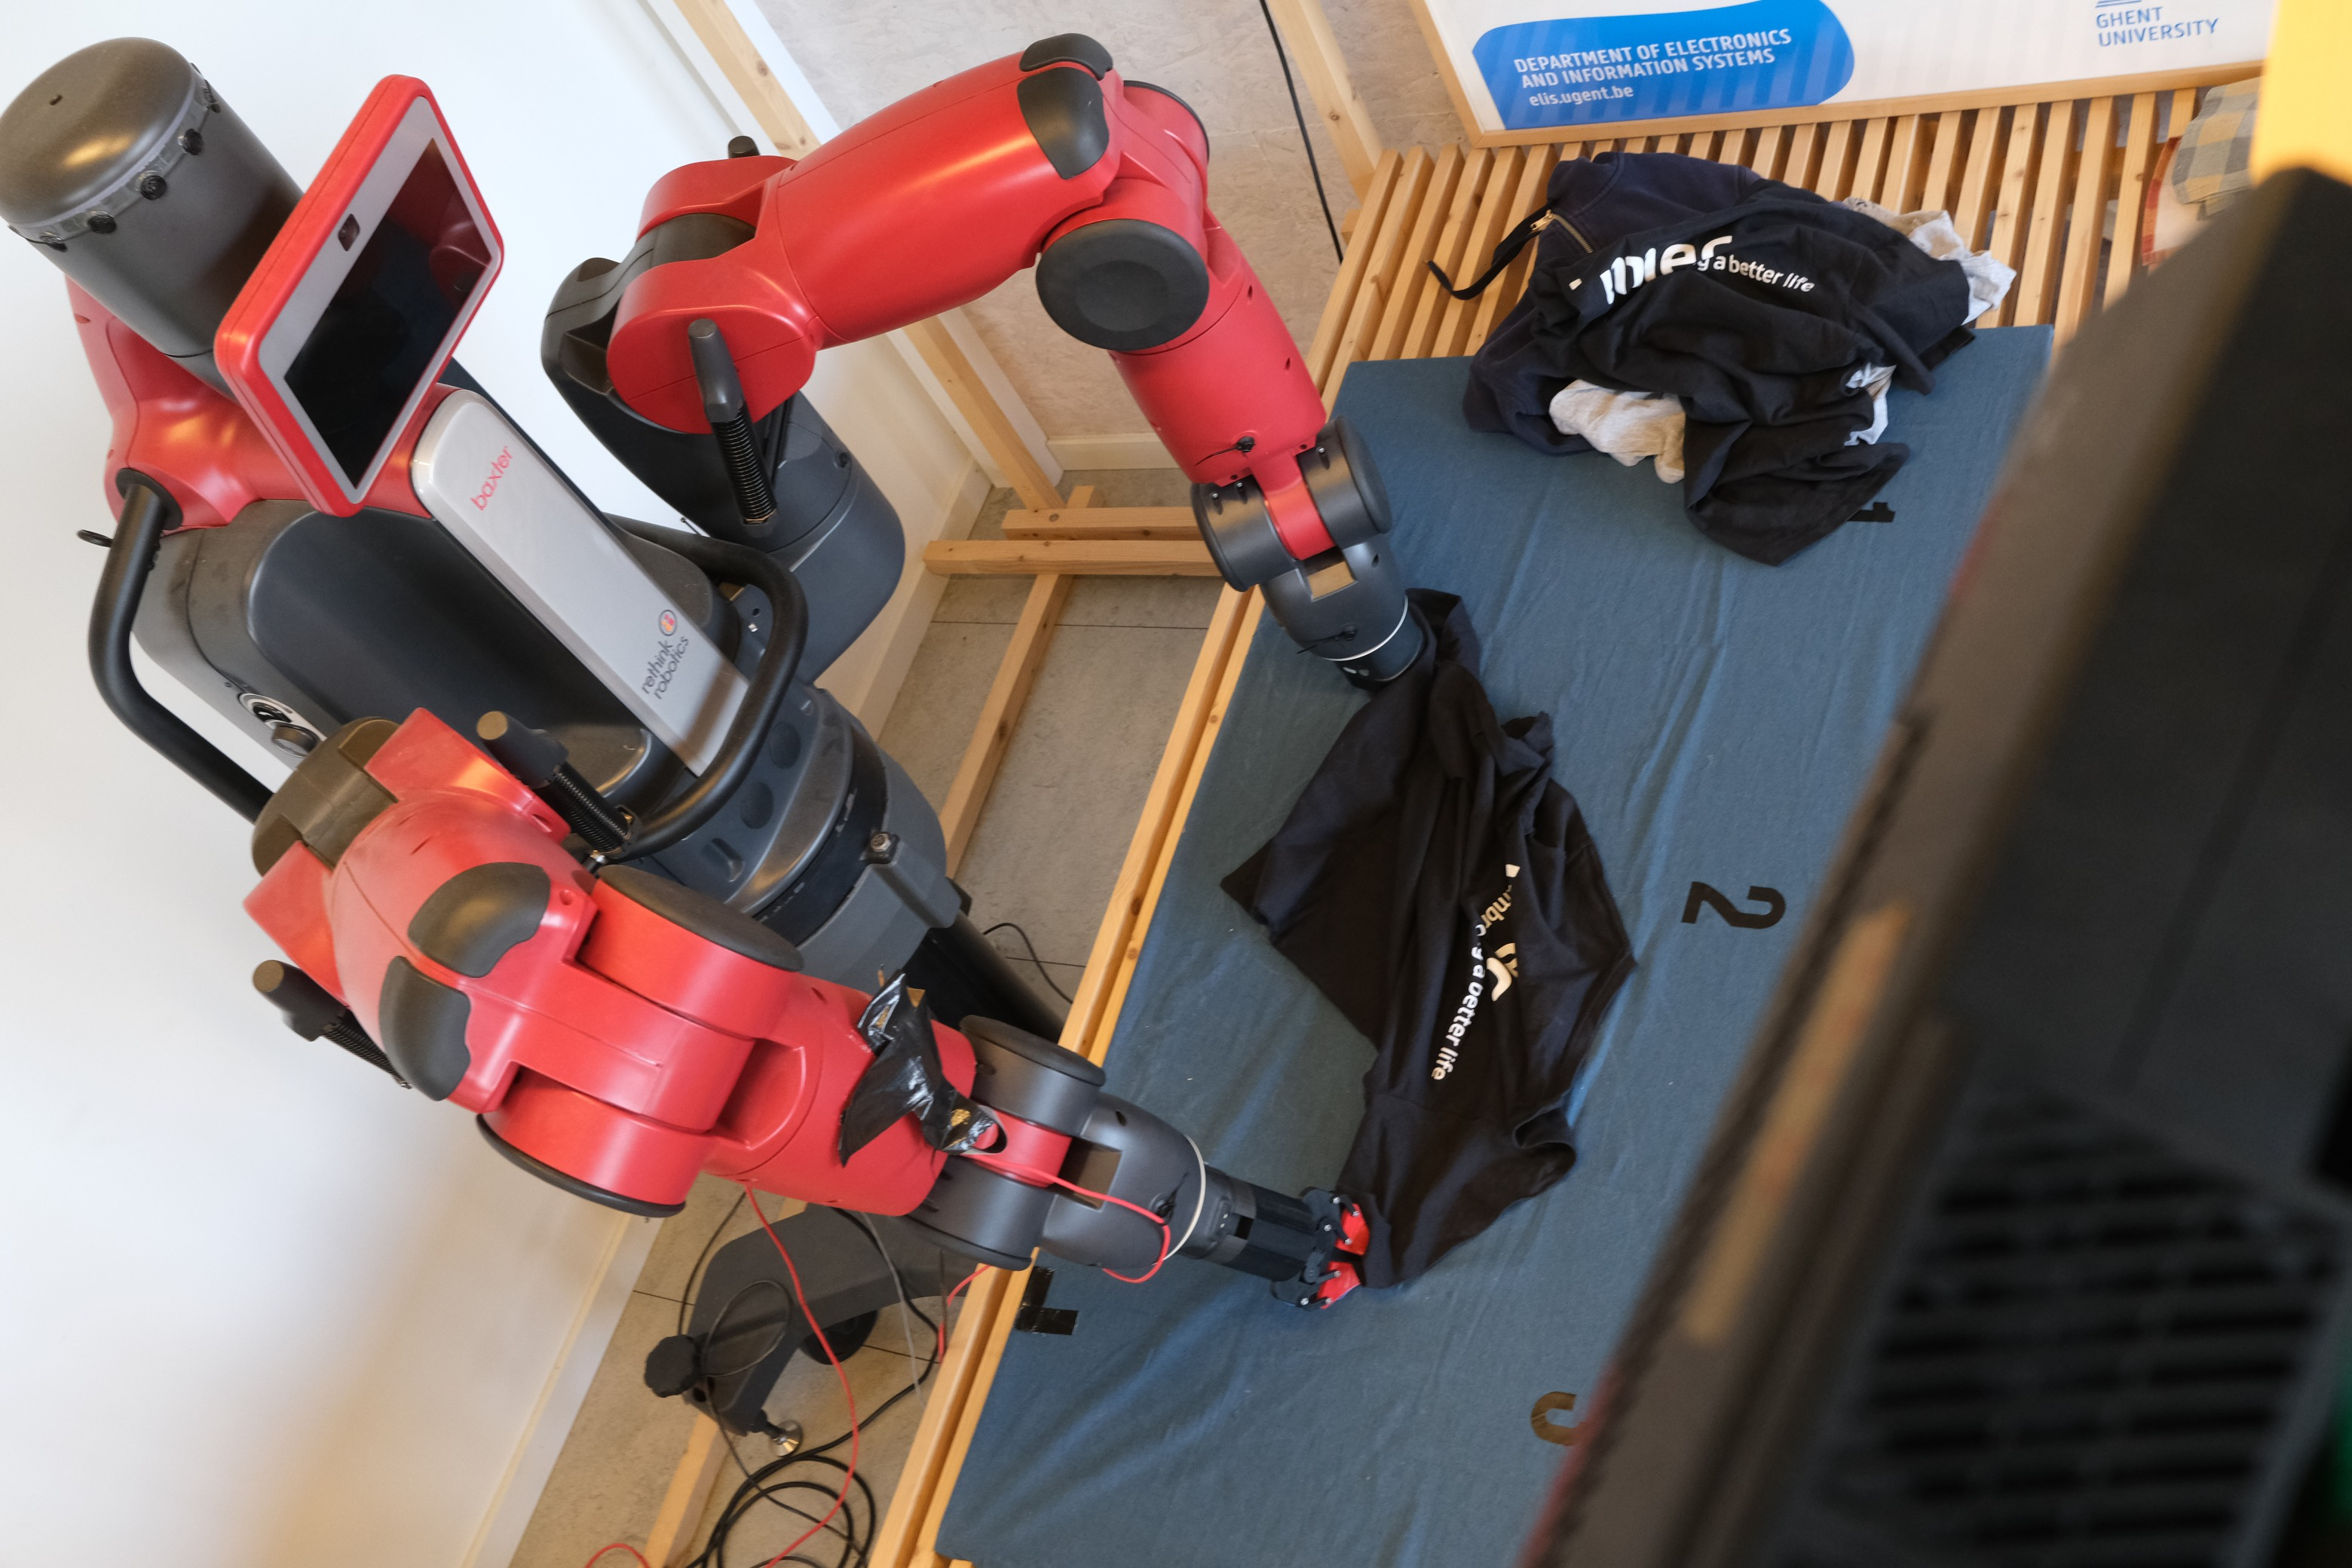
\includegraphics[width=\picMinWidth, height=\picMinHeight]{baxter_env_photo.JPG}};
    \node[below of=env, anchor=south, yshift=-1.25cm] (env_txt) {Image};

    \node[subblock, right= of env,align=center] (hog) {High-\\level\\features};
    \node[subblock, right= of hog,align=center] (mid) {Mid-\\level\\features};
    \node[subblock, right= of mid,align=center] (clf) {Object\\classifier};

    \node (perception box) [block,fit = (hog) (mid) (clf)] {};
    \node (perception box txt) [below of=perception box, anchor=south, yshift=-0.75cm] {Perception};

    \node[subblock,right=of perception box,align=center] (planning) {Planning\\module};
    \node[subblock,right=of planning,align=center] (control) {Control\\module};
    \node[subblock,right=of control,align=center] (baxter) {Motor\\commands};

    \draw [postSpacedArrow] (env) to node [] {} (perception box);
    \draw [postSpacedArrow] (hog) to node [] {} (mid);
    \draw [postSpacedArrow] (mid) to node [] {} (clf);
    \draw [postSpacedArrow] (perception box) to node [midway,text width=10mm,align=center,yshift=-0.5cm,text=gray,font=\tiny\linespread{0.1}\selectfont]{Class =\\shirt} (planning);
    \draw [postSpacedArrow] (planning) to node [] {} (control);
    \draw [postSpacedArrow] (control) to node [] {} (baxter);


\end{tikzpicture}
% \end{sidewaysfigure}
\end{document}
